\\\subsection{ADCS Components}
\FloatBarrier
\begin{figure}[hbt!]
  \centering
  \vspace{5mm}
  \subfloat[ Arcse Sagitta star tracker]{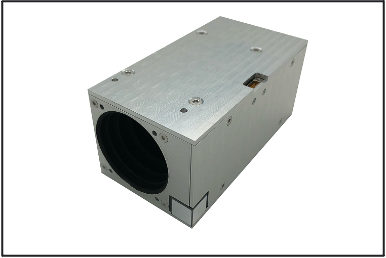
\includegraphics[width=0.5\textwidth,scale=0.8]{Images/ad1.png}\label{fig:ad1}}\hspace{5mm}
  \subfloat[nanoSSOC-D60]{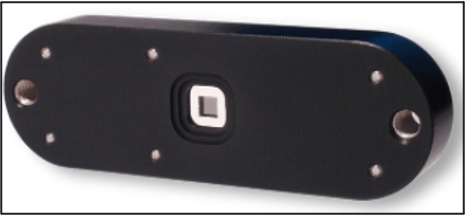
\includegraphics[width=0.4\textwidth,scale=0.8]{Images/ad2.png}\label{fig:ad2}}
%   \hfill% or \hspace{5mm} or \hspace{0.3\textwidth}
\\[1in]
  \subfloat[BiSon64-ET]{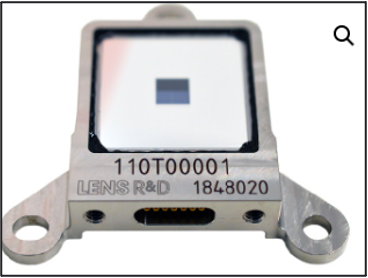
\includegraphics[width=0.5\textwidth,scale=0.8]{Images/ad3.png}\label{fig:ad3}}
 \hspace{4mm}
  \subfloat[Momentum Wheel]{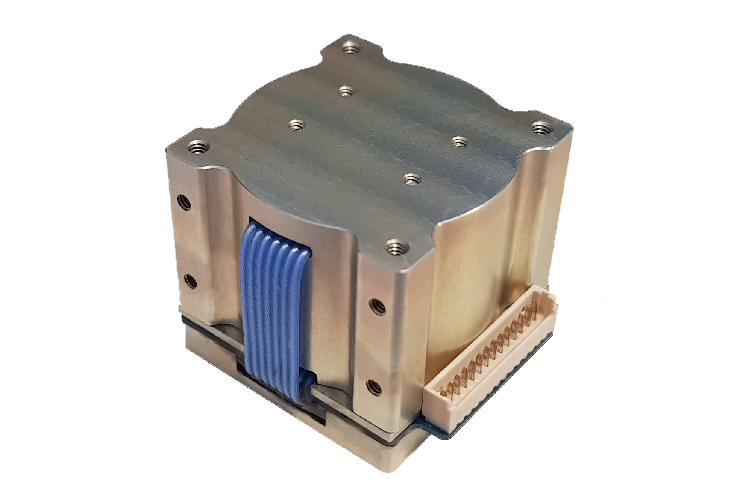
\includegraphics[width=0.5\textwidth,frame, scale=0.8]{Images/ad4.png}\label{fig:ad4}}
  \caption{ADCS Components }
  \label{fig:adcs}
\end{figure}
\newpage
\subsection{Electrical Components}
\begin{figure}[hbt!]
    \centering
    \subfloat[DHV-CS-10 CubeSat Solar Panel]{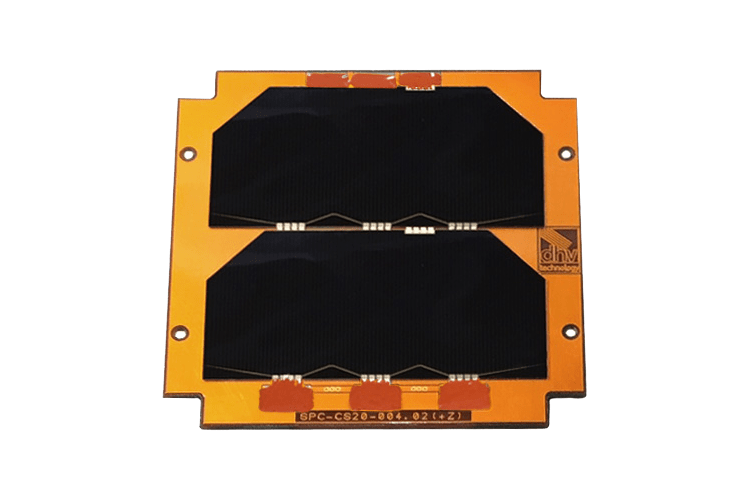
\includegraphics[width=0.4\textwidth,scale=0.8]{Images/DHVPanel.png}\label{fig:DHV}}\hspace{6mm}
    \subfloat[EXA Deployable Multifunction Solar Array]{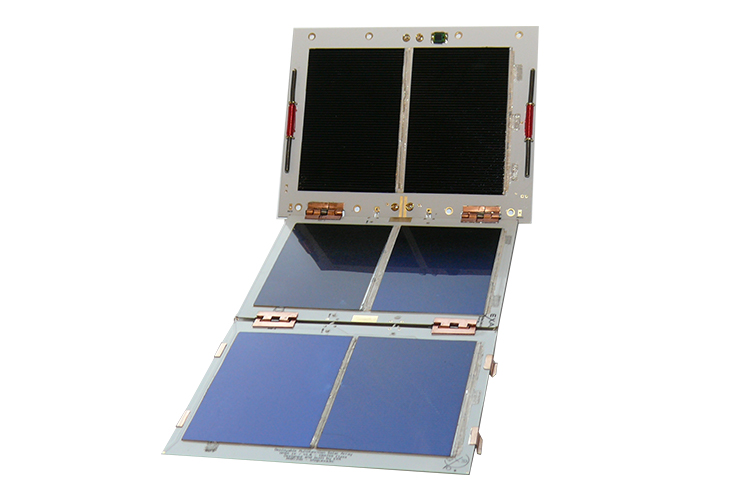
\includegraphics[width=0.4\textwidth,scale=0.8]{Images/EXAPanel.jpg}\label{fig:EXAp}}
    \subfloat[EXA BA01 Battery Array]{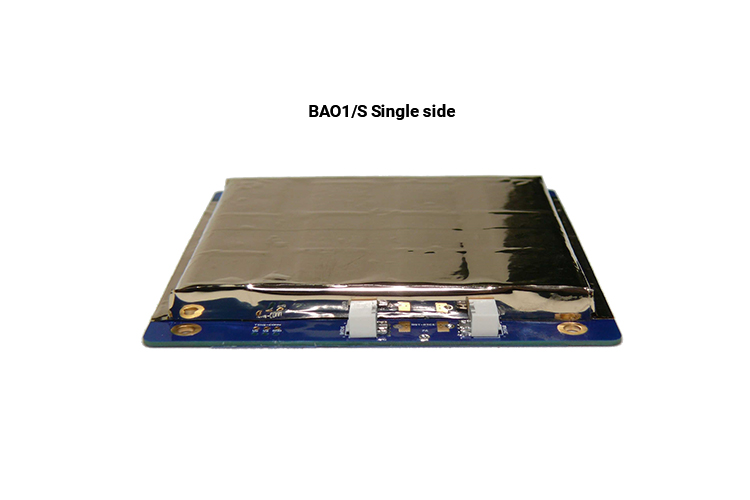
\includegraphics[width=0.4\textwidth,scale=0.8]{Images/EXABattery.jpg}\label{fig:EXAb}}
    \caption{Electrical Components}
    \label{fig:Elec}
\end{figure}
\\\subsection{CAD Drawings}
\begin{figure}[hbt!]
    \centering
    \subfloat[Frame: Side View]{{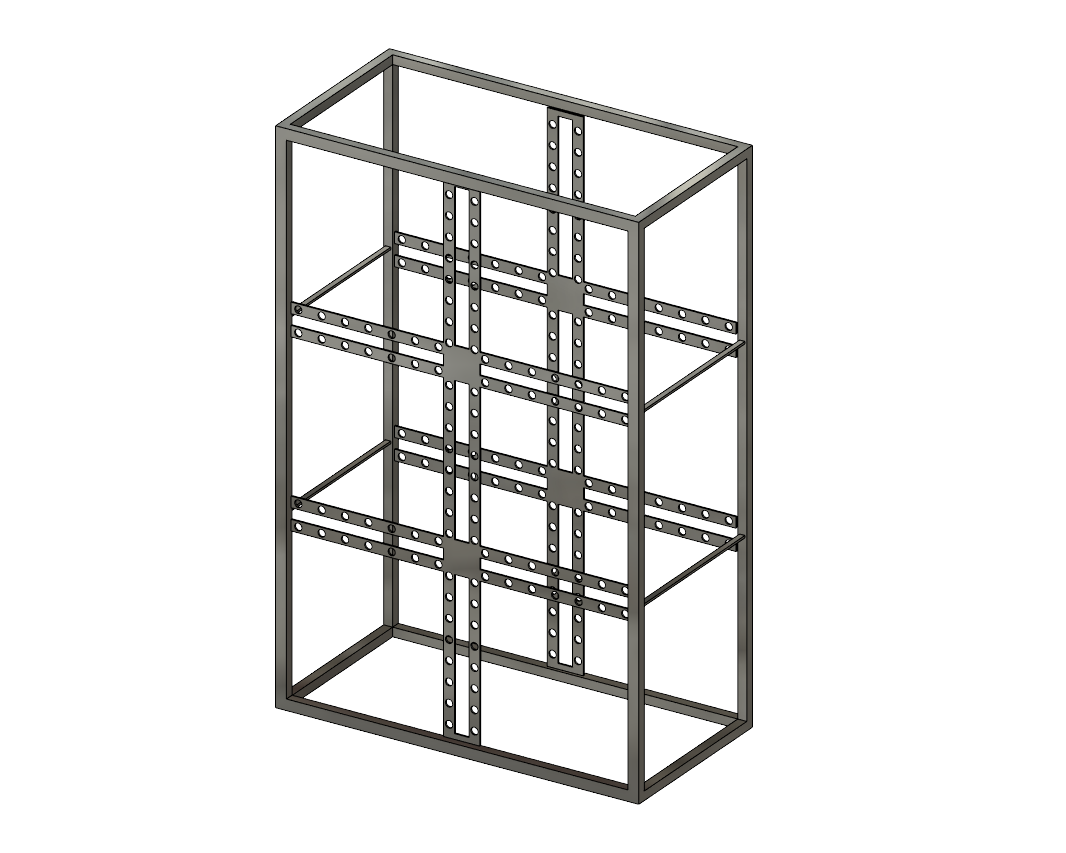
\includegraphics[width=8cm, scale=0.6]{Images/casing.png} }}\label{fig:p1}
    \qquad
    \subfloat[Frame: Iso View]{{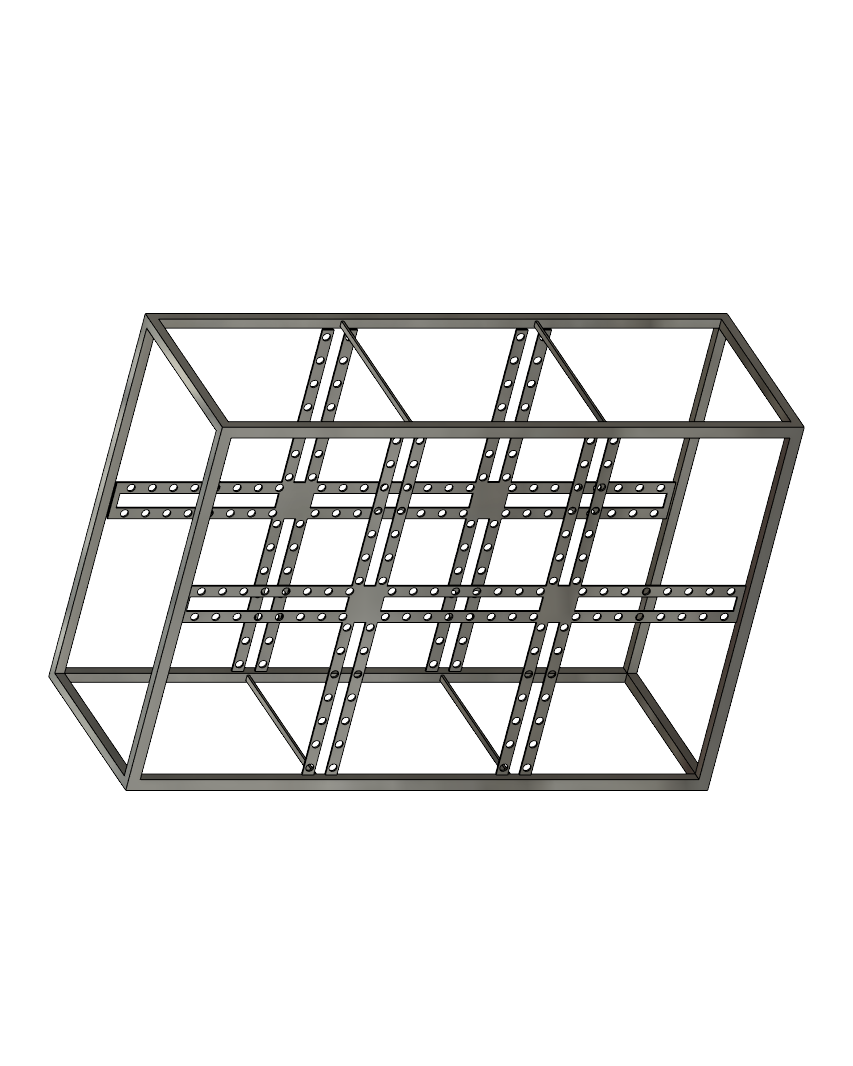
\includegraphics[width=7cm,scale=0.6]{Images/casing3.png} }}\label{fig:p2}
    \caption{Al7075-T651 Cubesat Frame}
    \label{fig:casing}
\end{figure}

\begin{figure}
    \centering
    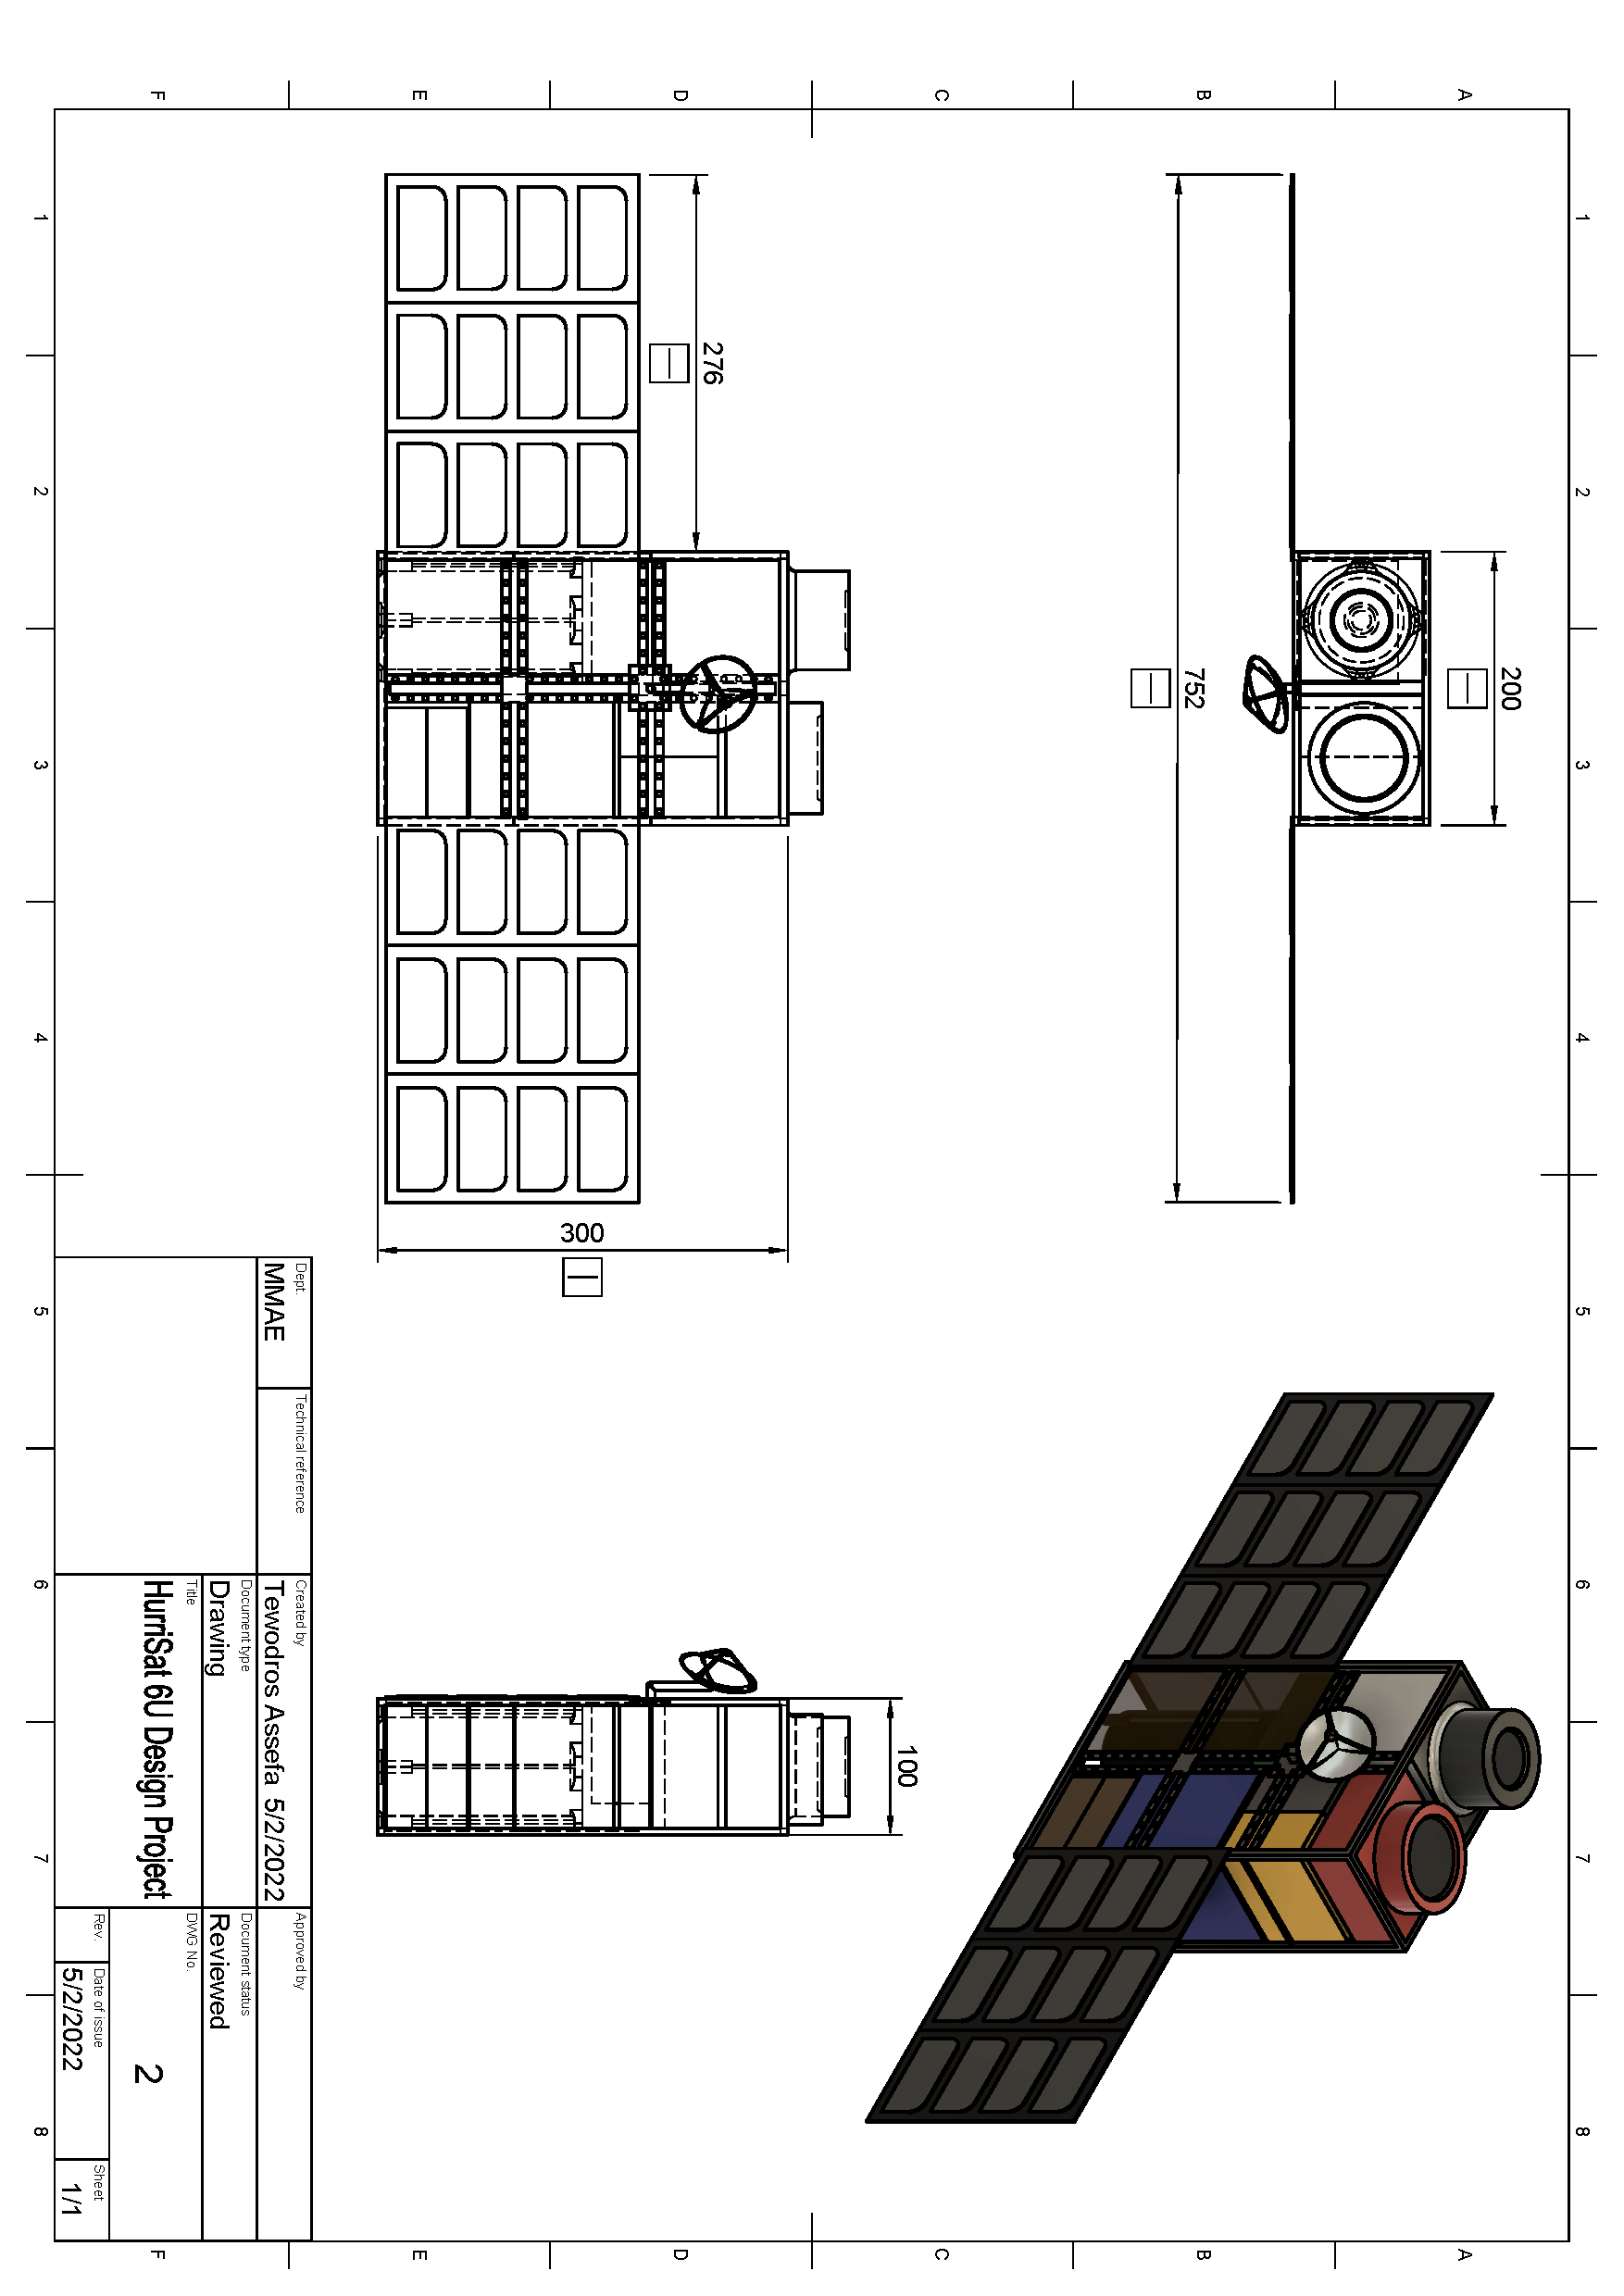
\includegraphics[width=\textwidth, keepaspectratio]{Images/CAD.pdf}
    \caption{Hurrisat CAD Drawing}
    \label{fig:drawing}
\end{figure}

\newpage
\subsection{Fact Sheet}
\begin{figure}[hbt!]
    \centering
    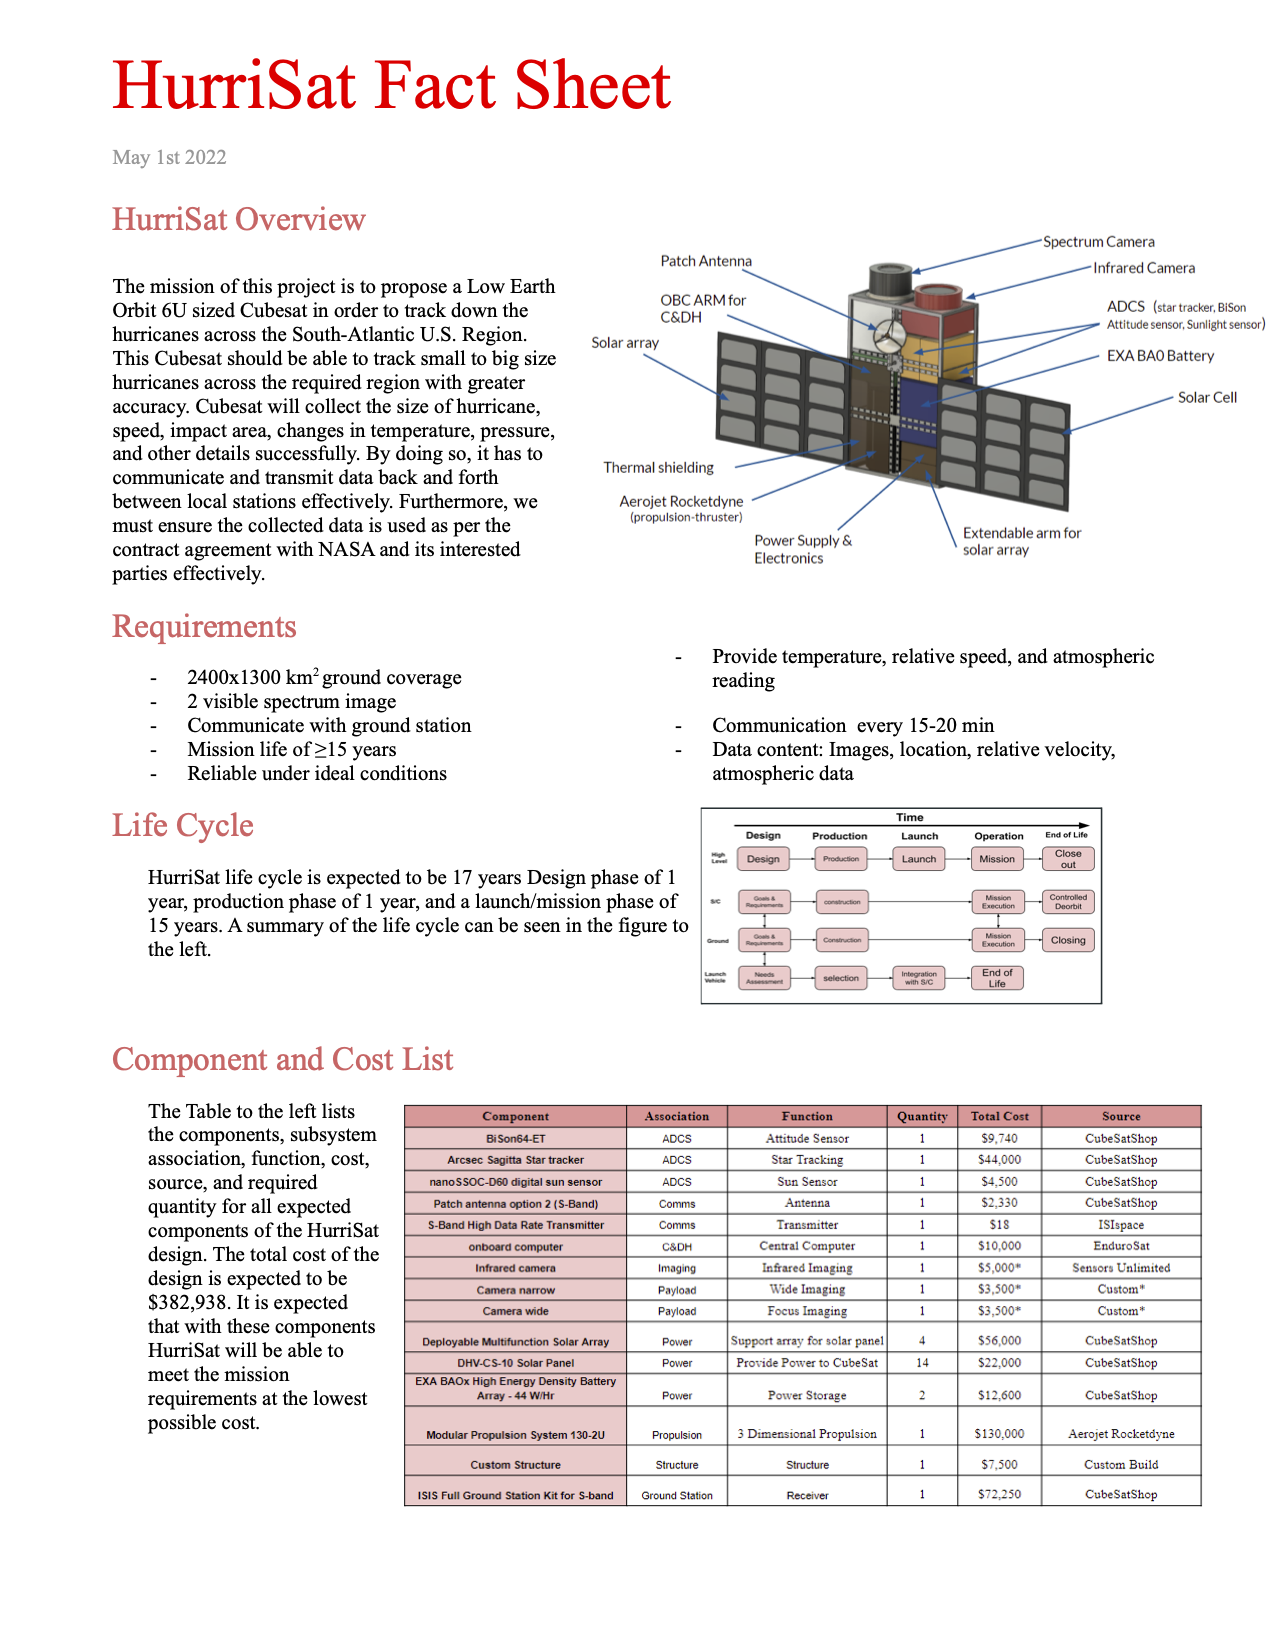
\includegraphics[width=\textwidth,frame]{Images/FactSheetHurriSat.png}
    % \caption{HurriSat Fact Sheet}
    \label{fig:Fact}
\end{figure}
\newpage
\subsection{Codes and Scripts} \label{codes}
\subsubsection{Script for Mass Sizing}
\begin{verbatim}
import numpy as np

pay_m=0.605 #initial mass of payload in kg using trade studies
dry_m=pay_m/(.3)
print("Dry mass is:", round(dry_m,4))
str_m=.11*dry_m
print("str_m=",round(str_m,3))
the_m=.02*dry_m
print("the_m=",round(the_m,3))
pow_m=.17*dry_m
print("pow_m=",round(pow_m,3))
tt_m=.15*dry_m
print("tt_m=",round(tt_m,3))
adcs_m=.08*dry_m
print("adcs_m=",round(adcs_m,3))
pro_m=.17*dry_m #we add three more to make it to 100%
print("pro_m=",round(pro_m,3))
mar_m=.1*dry_m
print("mar_m=",round(mar_m,3))
Tot_m=pay_m+str_m+the_m+pow_m+tt_m+adcs_m+pro_m+mar_m
print("Total Mass inlcuding the 10% margin (kg):", round(Tot_m,4))
\end{verbatim}

\subsubsection{Script for Delta V ($\Delta v_{design}$)}
\begin{verbatim}
import numpy as np
import sympy as sp
import math

def deltaV_design(phi, alpha, altitude, launchsite, losses):
    mu_e = 398600.5
    r_e = 6378.137
    V_bo = np.sqrt(mu_e/(r_e+altitude))
    beta = np.degrees(np.arcsin(np.cos(np.radians(alpha))/np.cos(np.radians(launchsite))))
    V_ls = 465.1*np.cos(np.radians(launchsite))/1000
    dV_gl = np.sqrt((2*mu_e*altitude)/(r_e*(r_e+altitude)))
    dV_needed = np.array([-V_bo*np.cos(np.radians(phi))*np.cos(np.radians(beta)), V_bo*np.cos(np.radians(phi))*np.sin(np.radians(beta)), V_bo*np.sin(np.radians(phi))]) + np.array([0, -V_ls, dV_gl])
    dV_design = np.linalg.norm(dV_needed) + losses
    return dV_design

alt=[800, 850, 900, 950, 1000, 1100, 1200]
alpha=[30, 32, 35, 40, 45, 52, 52] #inclination
phi=0 #circular orbit so flight path angle is assumed close to zero 
launchsite=28 #kenedy space center
loss=.9
for k in range(np.size(alt)):
    print("\nFor altitude = ", alt[k])
    for i in range(np.size(alpha)):
        print('If alpha(inclination) is:', alpha[i], 'then Vdeesign is:',round(deltaV_design(phi,alpha[i],alt[k],launchsite,loss),3))
\end{verbatim}
\subsubsection{Script for Attitude Determination and Control}
\begin{verbatim}
import numpy as np
import sympy as sp
import math

Imax = 55
Imin = 30
MomentArm = 0.3
ResidualDipole = 2
FrontalSA = 1
mu_e = 398600.5
r_e = 6378.137
Altitude = 700
R = Altitude + r_e
magLat = 10
VrelativeX = -1.006320
VrelativeY = -1.225255
VrelativeZ = 7.427699
Vrelative = np.sqrt(VrelativeX**2 + VrelativeY**2 + VrelativeZ**2)

Tg = 3 * mu_e * (Imax - Imin) / (R**3)
print(f'The maximum gravity gradient torque per degree is {Tg}')

AD = 1.47e-13
Cd = 3
F = 0.5 * AD * Cd * FrontalSA * Vrelative
Ta = MomentArm * F
print(f'The magnitude of the maximum drag torque is {Ta}')

B0 = 3.12e-5
B = B0 * ((r_e / R)**3) * np.sqrt(1 + (3 * (np.sin(np.radians(magLat))**2)))
Tm = ResidualDipole * B
print(f'The magnitude of the maximum magnetic torque is {Tm}')

Fs = 1378
c = 3e8
As = 
q = 0.6
i = 
F2 = (Fs * As * (1 + q) * np.cos(np.radians(i))) / c
Ts = MomentArm * F2
print(f'The magnitude of the maximum solar pressure torque is {Ts}')
\end{verbatim}

\newpage
\subsection{Keywords}
AF-M315E: Hydroxyl Ammonium Nitrate fuel/oxidizer blend\\
ADCS: Attitude Determination and Control System\\
ADN: Ammonium dinitramide\\
Al7075: Alummunim Alloy\\
BPSK: Binary Phase-shift keying\\
CSLI: Cubesat Launch Initiative\\
GPS: Global Positioning System\\
S-Band: a radio frequency band from 2 to 4 GHz\\
LiDAR: laser imaging, detection, and ranging\\
MLI: Multi-layer insulation\\
MPS: Main Propulsion Subsystem\\
NASA: National Aeronautics and Space Administration\\
NESDIS: National Environmental Satellite, Data, and Information Service\\
NOAA: National Oceanic and Atmospheric Administration\\
NWPC: National Weather Prediction Center\\
NWS: National Weather Service\\
OBC: On board computer\\
PSK: Phase-shift keying\\
STK: Space Mission Toolkit by AGI Solutions\\
TT\&C: Telemetry, Tracking and Command\\ 
\subsection{List of Tables}
Table \ref{Tab:hss}. Hurricane Severity\\
Table \ref{Tab:sh}. Stakeholders\\
Table \ref{Tab:rd}. Risk Definitions\\
Table \ref{Tab:rcg}. Risk Color-grading\\
Table \ref{Tab:tpr}. Risk Assessment\\
Table \ref{Tab:ms}. Mission Life Summary\\
Table \ref{Tab:lvc}. Launch Vehicles Compared\\
Table \ref{Tab:hoh}. Transfer Values\\
Table \ref{Tab:pc}. Payload Characteristics\\
Table \ref{Tab:ps}. Power Sizing\\
Table \ref{Tab:ms}. Mass Sizing\\
Table \ref{Tab:dv}. $\Delta{V_{design}}$\\
Table \ref{Tab:comms}. Communications Table\\
Table \ref{Tab:obc}. OBC Data Handling\\
Table \ref{Tab:Prop}. Propellant Comparison\\
Table \ref{Tab:alloy}. Aluminum Alloy Comparison\\
Table \ref{Tab:msc}. Mission Success Criteria\\
Table \ref{Tab:ms}. Mission Risks\\

\subsection{List of Figures}
Figure \ref{fig:ssreq}. Subsystem Requirements and Constraints\\
Figure \ref{fig:manplan}. Mission Analysis\\
Figure \ref{fig:graph}. Trade Studies\\
Figure \ref{fig:orbiGC}. HurriSat Orbit and Ground Coverage\\
Figure \ref{fig:march}. Mission Architecture\\
Figure \ref{fig:timelin}. HurriSat Timeline\\
Figure \ref{fig:diagram}. Block Diagram\\
Figure \ref{fig:hohfig}. Hohmann Transfer simulated using STK\\
Figure \ref{fig:cameras}. Required Cameras\\
Figure \ref{fig:cost}. Cost Budget
Figure \ref{fig:hurrisat}. HurriSat and its Components\\
Figure \ref{fig:config}. HurriSat Launch Configuration\\
Figure \ref{fig:comms}. Communication Mechanism\\
Figure \ref{fig:obc}. On Board Computer\\
Figure \ref{fig:thermal}. Thermal Limitations\\
Figure \ref{fig:prop}. Propulsion System\\
Figure \ref{fig:modal}. Modal analysis of structure \\
Figure \ref{fig:rplot}. Risk Control \\
Figure \ref{fig:alter}. Alternative frames considered\\
Figure \ref{fig:adcs}. ADCS Components\\
Figure \ref{fig:Elec}. Electrical Components\\
Figure \ref{fig:casing}. Al7075-T651 Cubesat Frame\\
Figure \ref{fig:drawing}. Hurrisat CAD Drawing\\
\newpage